Die kontinuierliche Wavelettransformation 
\begin{equation}
\Wave f (a,b)
=
\langle f,\psi_{a,b}\rangle
=
\frac{1}{\sqrt{|a|}}\int_{-\infty}^\infty f(t)\,
\overline{\psi}\biggl(\frac{t-b}{a}\biggr)\,\mathrm{d}t
\end{equation}
kann mittels FFT sehr effizient berechnet werden.
Die Wavelettransformation entspricht nämlich einer Faltung.
Deren Berechnung wird im Frequenzbereich zu einer einfachen Multiplikation
\begin{equation}
\Wave f(a,b)
= \mathcal{F}^{-1}\bigl\lbrace\hat{f}(\omega) \sqrt{|a|}\, \overline{\hat{\psi}}(a\omega)\bigr\rbrace.
\end{equation}
Besonders interessant ist diese Berechnung mit Wavelet, die eine geschlossene, analytische Form im Frequenzbereich besitzen, etwa das Haar- oder das Gabor-Wavelets.
Wie alle reellen Wavelets erlauben auch diese zwei nicht, Phase und Amplitude getrennt zu betrachten.
Eine Detektion der momentanen Signalfrequenzen wird dadurch erschwert.

Durch den \emph{Auslöschungsoperator}
\[
	\Ana\, \colon L^2(\mathbb R) \to L^2(\mathbb C)
	\quad\colon\quad
	\psi \mapsto \frac{1 + i\Hilb\,}{\sqrt 2}\psi
\]
können wir jedoch aus jedem, reellen Wavelet ein \emph{analytisches Wavelet} erstellen, welches dem Original sehr ähnlich ist, jedoch eine Trennung von Phase und Amplitude erlaubt.
Dadurch ist es möglich, im erhaltenen Bild dem Punkt des maximalen Betrags zu folgen.
Die \emph{dominanten Frequenz} des Wavelets erlaubt eine Interpretation dieser Maximas als Momentanfrequenz.

Durch den Operator $\Ana\,$ gelangten wir vom Gabor- zum Morlet-Wavelet, welche durch den Parameter $\sigma$ erlaubt, Zeit- und Frequenz-Lokalisierung gegeneinander auszuspielen.
Für maximale Lokalisierung in der Zeit, etwa für Sprungstellen, haben wir das analytische Haar-Wavelet berechnet.

Zum Schluss haben wir gesehen, dass durch die FFT als Algorithmus zur Berechnung von Fourierreihen immer eine \emph{zirkuläre Faltung} entsteht.
Dies führt zu Artefakten am Rande, welche sich durch \emph{Signal Padding} reduzieren lassen.
Eine generelle Lösung für dieses Problem gibt es jedoch nicht.

Zum Abschluss folgen nun noch ein paar weitere Bilder von Wavelettransformationen.
Interessante Merkmale sind in den Bildlegenden hervorgehoben.


\begin{figure}
	\centering
	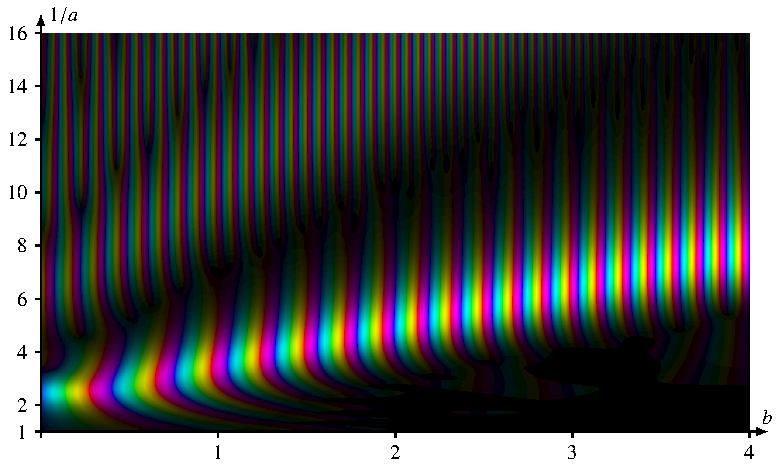
\includegraphics[width=\linewidth, keepaspectratio]{papers/complex/images/add_rs_chirp_morlet.pdf}
	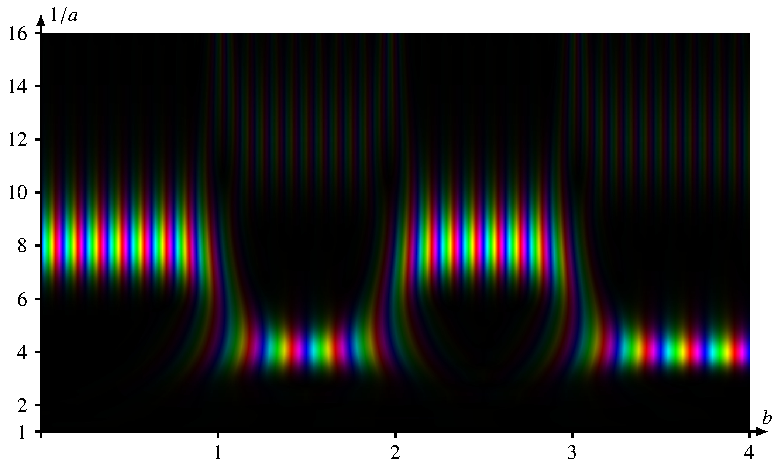
\includegraphics[width=\linewidth, keepaspectratio]{papers/complex/images/add_rs_square_morlet.pdf}
	\caption{Wavelettransformation mit dem Morlet-Wavelet und einer Rechteck- anstelle der Cosinus-Schwingung.
		In beiden Bildern ist die dritte Harmonische gut sichtbar.}
\end{figure}

\begin{figure}
	\centering
	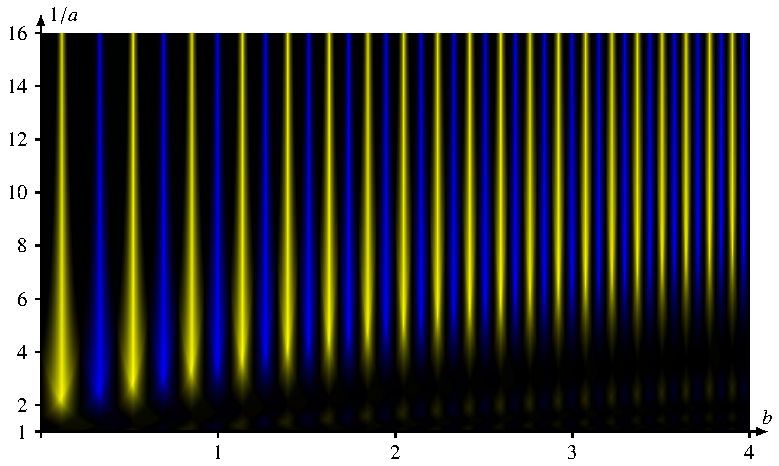
\includegraphics[width=\linewidth, keepaspectratio]{papers/complex/images/add_rs_chirp_haar.pdf}
	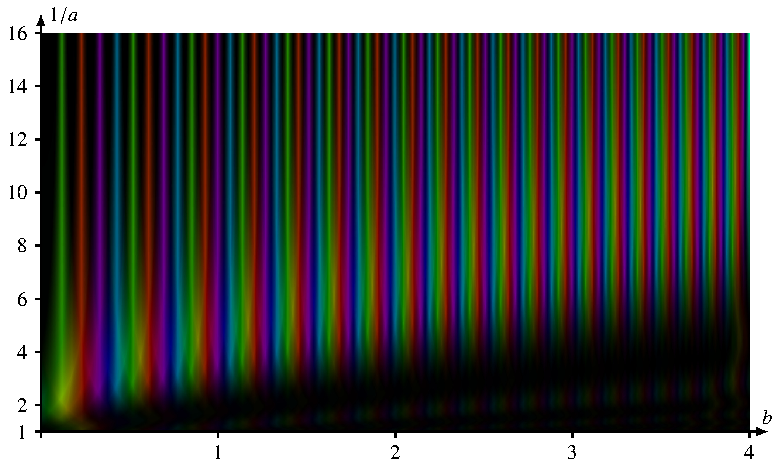
\includegraphics[width=\linewidth, keepaspectratio]{papers/complex/images/add_cs_chirp_haar.pdf}
	\caption{Wavelettransformation mit dem Haar-Wavelet. 
		Im oberen Bild wurde die Cosinus-Schwingung durch ein Rechteck-Signal mit $\pm 1$ ersetzt, im unteren Bild durch ein ``komplexes Rechtecksignal'' mit den Werten $\lbrace1, i, -1, -i\rbrace$.
		Das Haar-Wavelet entspricht für grosse Werte von $1/a$ einer Art Ableitung (vorheriger minus nachfolgender Mittelwert) und eignet sich deshalb besonders gut, um Sprünge im Signal zu finden.}
\end{figure}

\begin{figure}
	\centering
	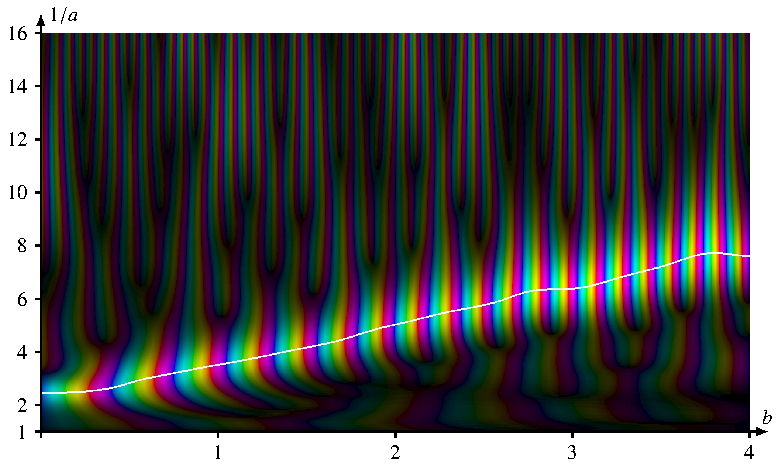
\includegraphics[width=\linewidth, keepaspectratio]{papers/complex/images/add_nc_chirp_haar.pdf}
	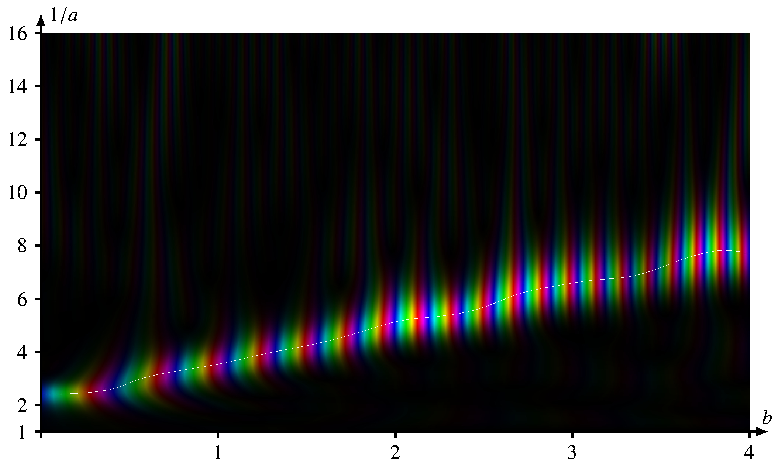
\includegraphics[width=\linewidth, keepaspectratio]{papers/complex/images/add_nc_square_haar.pdf}
	\caption{Wavelettransformation der beiden Beispielsignale mit dem Morlet-Wavelet. 
		Den Signalen wurde zusätzlich ein weisses Rauschen mit $\mu = 0$ und $\sigma = 1$ überlagert (\SI{0}{\decibel} SNR).
		Dies zeigt die Stärke der Wavelets in der Gegenwart von Rauschen.}
\end{figure}
